
%%%%%%%%%%%%%%%%%%%%%%%%%%%%%%%%%%%%%%%%%%%%%%%%%%%%%%%%%%%%%%%%%%%%%%%
%                          Thesis Appendix A                          %
%                       Numerical Optimization                        %
%%%%%%%%%%%%%%%%%%%%%%%%%%%%%%%%%%%%%%%%%%%%%%%%%%%%%%%%%%%%%%%%%%%%%%%

\chapter{Numerical Optimization: Introduction}
\label{chapter:optimization}

\nomenclature[x-R]{$\mathbb{R}$}{Real space}
\nomenclature[x-S]{$\mathit{S}$}{Variable space}
\nomenclature[x-M]{$\mathcal{M}$}{A Manifold}
\nomenclature[x-T]{$T_x\mathcal{M}$}{The tangent space of manifold $\mathcal{M}$ at point x}
\nomenclature[a-F]{$F$}{The set of linearized feasible directions}
\nomenclature[a-f]{$f$}{Objective function}
\nomenclature[a-c]{$c_i$}{Constraint function}
\nomenclature[a-x]{$x$}{Optimization variable}
\nomenclature[a-xstar]{$x^*$}{Solution of the optimization problem}
\nomenclature[a-E]{${E}$}{Set of index for which constraints are equality constraints}
\nomenclature[a-I]{${I}$}{Set of index for which constraints are inequality constraints}
\nomenclature[x-L]{$\mathcal{L}(x,\lambda)$}{Lagrangian function of the optimization problem}
\nomenclature[G-o]{$\Omega$}{Feasible set}
\nomenclature[z-st]{s.t.}{subject to}
\nomenclature[z-KKT]{KKT}{Karush-Kuhn-Tucker first order optimality conditions}
\nomenclature[z-LICQ]{LICQ}{Linear Independence Constraints Qualification}
\nomenclature[z-QP]{QP}{Quadratic Programming}
\nomenclature[z-IQP]{IQP}{Inequality constrained Quadratic Programming}

\graphicspath{{Appendix1-Optim/Figs/}}

%{{{SECTION: LIST OF CONTRIBUTIONS
%\section{List of contributions}
%\begin{itemize}
  %\item \sout{Introduction to optimization}
  %\item \sout{Notions of unconstrained optimization}
  %\item \sout{Notions of Constrained Optimization}
  %\item \sout{KKT}
  %\item Line Search
  %\item Trust Region
  %\item Filter
  %\item Merit function
  %\item SQP
  %\item Restoration phase
  %\item \sout{Hessian Approximation: BFGS, SR1}
%\end{itemize}
%}}}
\section{Introduction}
In modern science, optimization has an important place.
Mechanical engineers optimize the shape of structural parts.
Investors optimize the profit of a portfolio while minimizing the risks of loss.
Chemists optimize the efficiency and speed of reactions.
When it comes to robotics, optimization is widely used.
From the design of a robot to its actuation.
Any positioning of a robot requires the computation of the articular parameters of each joint of the robot, finding such parameters might be possible by using analytical methods for simple robots, but for robots as complex as humanoid robots, it is not possible.
Most often, an optimization process is used.

The goal of an optimization algorithm is to find an optimal solution $x^*$ to a problem.
Optimal in the sense that the solution is an optimum of a given objective function $f$.
And solution of a problem in the sense that is satisfies a set of $m$ constraints $\{c_i,\ i\in [1,m]\}$.
Both the constraints and the objective function are defined on the variable space $\mathit{S}$, which is the space in which the variable $x$ lives and in which we search a solution $x^*$ to our problem.

In order to present the principles of optimization, in this chapter we will always consider that the variable space is $\mathit{S}=\mathbb{R}^n$.
We first consider unconstrained problems.
That type of problem will not be used in the rest of our dissertation, therefore, we will just present them shortly.
We will then focus on constrained optimization problems and the numerous methods used in their resolution.
We will particularly detail one specific constrained problem resolution algorithm that is the Sequential Quadratic Program (SQP).
The extension of those methods to solving problems on more complex variable spaces that are the non Euclidean manifolds is the topic of Chapter~\ref{chapter:optimization_on_noneuclidean_manifolds}.

This Appendix does not pretend to give a fully detailed overview of numerical optimization methods, it gives the reader a quick overview of some key principles.
For more detailed information, we invite the reader to refer to the excellent books that we took inspiration from to write this chapter~\cite{nocedal:book:2006, bonnans:book:2003, boyd2004convex}.

\section{Unconstrained Optimization}

An unconstrained optimization problem consists in minimizing an objective function without any constraint.
This problem, denoted $\mathcal{P}$, can be formulated as follows:

\begin{equation}
  \minimize_{x\in\mathbb{R}^n}\ {f(x)}
\label{eq:unconstrainedOptim}
\end{equation}

The classical approach to solve $\mathcal{P}$ is to use an iterative algorithm, starting from an initial guess $x_0$, and converging toward the solution $x^*$.
A very basic optimization scheme is Algorithm~\ref{alg:basic_optim}.

\begin{algorithm}
\begin{algorithmic}
  \State{Starting from an initial guess $x_0$}
  \While{Convergence condition not met}
  \State{Compute descent direction $d_k$}
  \State{Compute step length $t_k$}
  \State{Update $x_{k+1}\leftarrow x_k + t_k d_k$}
  \EndWhile{}
  \caption{Basic optimization scheme}
\label{alg:basic_optim}
\end{algorithmic}
\end{algorithm}

The objective function is not necessarily completely known, in the sense that we cannot always have an explicit formula. Often, the function $f$ is computed by another program that is able to compute $f(x)$, $\nabla_x f(x)$ and sometimes $\nabla_{xx} f(x)$ for a given value of $x$.
In order to have an efficient algorithm, we need to avoid any unnecessary computation of $f(x)$ and its derivatives.
We denote the values taken by $x$ along the iterations as $x_0$, $x_1$, $x_2$,\ldots $x_i$.
And $f(x_i)$ is denoted $f_i$.

Since our knowledge of the objective function is only partial, it would not be possible to guarantee that a point $x^*$ is a global solution:

\begin{equation}
  \text{$x^*$ is a global solution of $\mathcal{P}$ on $\mathit{S}$ } \equiv \forall x \in \mathit{S}, f(x^*) \leq f(x)
\end{equation}

Though, we can find a local solution $x^*$ of $\mathcal{P}$ (a local minimizer of $f$): such that there exist a neighborhood $\mathit{N}$ of $x^*$ where $\forall x\in \mathit{N}$, $f(x^*) \leq f(x)$.
Or even a strict local minimizer of $f$: such that there exist a neighborhood $\mathit{N}$ of $x^*$ where $\forall x\in \mathit{N}$, $f(x^*) < f(x)$.
That is the kind of solution that we are looking for and that our algorithms should find.

Under the assumption that the objective function is smooth and sufficiently continuous ($\mathcal{C}^2$), then we have the following sufficient conditions for the optimality of $x^*$ as presented in~\cite{nocedal:book:2006}:

\begin{theorem}
  If $\nabla^2f$ is continuous in an open-neighborhood of $x^*$ and that $\nabla f(x^*)=0$ and $\nabla^2 f(x^*)$ is positive definite.
  Then $x^*$ is a strict local minimizer of $f$.
\label{optimalityTheorem}
\end{theorem}

\subsection{Globalization methods (Section NEEDS TO BE REWRITTEN)}

During the resolution of an optimization problem, the algorithm will generate a
sequence of iterates $x_k$ starting from the initial iterate $x_0$ (Which is
usually provided by the user). During the step $k$ of the optimization process,
the solver, the current point is $x_k$ and we try to find $x_{k+1}$ such that
$f(x_{k+1}) < f(x_k)$. There are several strategies to do that but we will only focus
on 2 of them that are the most popular, the line-search and trust-region
methods.

\subsubsection{The Line-Search Strategy}
In the Line-Search strategy, given a point $x_k$, a descent direction $p_k$ from this
point is chosen and then a length of step is calculated to minimize the
following 1-dimensional problem:
\begin{align}
  \minimize_{\alpha \in \mathbb{R}^+} f(x_k + \alpha.p_k)
\label{eq:lineSearchNLP}
\end{align}

Once the best value of $\alpha$ has been found, the next iterate is computed:
$x_{k+1} = x_{k} + \alpha p_k$ and the same process is repeated until a
satisfying solution is found.

It is not always necessary to find the optimal value of $\alpha$, especially if
that is expensive. Indeed, $\alpha$ is only used to calculate the next iterate,
from which another $p_k$ and $\alpha$ will be calculated. And in the end, the
imprecision on the computation of $\alpha$ will be erased in the other steps of
the resolution.

There are several ways to choose a descent direction from an iterate $x_k$. The
most obvious one is probably the steepest descent direction $-\nabla f_k$. This
method provides the direction along which f decreases most rapidly and only
requires the evaluation of the first derivative of $f$, but that method can
become extremely slow on complicated problems. Another popular approach is the
Newton method, in which the objective function is approximated to the second
order

\begin{equation}
  f(x_k+p) = f_k + p^T\nabla f_k + p^T\nabla^2f_k p
\end{equation}

Then the chosen descent direction is the optimum of that approximated function,
the Newton direction.
\begin{equation}
  p^N_k = -{(\nabla^2 f_k)}^{-1} \nabla f_k
\end{equation}
The choice of this descent direction implies that the $\nabla^2f_k$ is positive
definite, in which case an adaptation of the definition of $p_k$ is required. Or
an approximation $B_k$ of $\nabla^2f_k$ that guaranties definite positiveness can be
used. For example, the symmetric-rank-one (SR1) formula and the BFGS (Broyden,
Fletcher, Goldfarb, Shanno) formula. Then the step becomes

\begin{equation}
  p_k = -B_k^{-1}\nabla f_k
\end{equation}

\subsubsection{The Trust-Region Strategy}
\label{ssec:the_trust_region_strategy}
The Trust-Region Strategy works in an opposite way than the line-search one in
the sense that during a line-search step, a direction is chosen, and based on
that direction, a step-length is chosen. Whereas with a Trust-Region approach, a
maximum step-length is chosen, and based on it, the descent direction and length
are chosen.
The principle of the trust region is that along the optimization process, a
model of the problem is constructed and enriched at every step and at each step,
the next iterate is the optimum of the model, with the constraint that the step
to get there lies inside the trust-region. For example, let us consider that
the trust region is a sphere of center $x_k$ and radius $\rho_k$, then the
constraint on $p_k$ is $\|p_k\| \leq \rho_k$. A usual model to take for the
objective function is the quadratic model with approximated Hessian
\begin{equation}
  m_k(p) = f(x_k+p) = f_k + p^T \nabla f_k + p^T B_k p
\end{equation}
And the optimization problem to solve at each step of the optimization is

\begin{align}
  \minimize_{p} & \quad f_k + p^T \nabla f_k + p^T B_k p \nonumber\\
\text{s.t.}&
\quad \|p\| \leq \rho_k
\label{eq:trustRegionNLP}
\end{align}

Once the solution $p_k$ to this quadratic problem is found, its quality is
estimated by evaluating the value of $f(x_k+p_k)$. If the actual decrease of $f$
is satisfying (compared to the decrease predicted by the model) then the step is
accepted and the size of the trust-region can be increased. Otherwise, the step
is refused, the trust-region radius is reduced and a new step from $x_k$ is
computed on that smaller trust region.

\section{Constrained Optimization}

Solving a constrained optimization problem consists in minimizing a cost function while satisfying a set of constraints.

A general formulation for such problems (that we denote $\mathcal{P}$) is:

\begin{equation}
  \label{formulation_NLCP}
  \mathcal{P} \equiv
  \left\{
  \begin{array}{l}
    \minimize\limits_{x\in\mathbb{R}^n}{f(x)}\\
    \text{ s.t. }
    \left\{
    \begin{array}{l}
      c_i(x) = 0,\ \forall i\in{E}\\
      c_i(x) \geq 0,\ \forall i\in{I}\\
    \end{array}
    \right.
  \end{array}
  \right.
\end{equation}

Where $f$ and $c_i$ are real valued functions on a subset of $\mathbb{R}^n$.
$f$ is the objective function, and the $c_i$ are the constraint functions.
${I}$ and ${E}$ are sets of index such that $c_i,\ i\in{E}$ are the equality constraints, and $c_i,\ i\in{I}$ are the inequality constraints.

We define the feasible set $\Omega$ that contains all the feasible points (points satisfying the constraints) of $\mathcal{P}$.

\begin{equation}
  \Omega = \left\{ x\in \mathbb{R}^n:\ \forall i\in {E},\ c_i=0,\ \forall i\in{I},\ c_i \geq0\right\}
\end{equation}

The formulation~\ref{formulation_NLCP} can then be rewritten as:
\begin{equation}
  \label{formulation_NLCP_compact}
  \mathcal{P} \equiv \minimize_{x\in\Omega}{f(x)}
\end{equation}

In the general case, the problem~\ref{formulation_NLCP_compact} has multiple local solutions.
And finding the global minimizer of $f$ in $\Omega$ is a difficult problem that we do not treat in this thesis.
Our goal is to find a local minimizer $x^*$ of $f$ in $\Omega$.

\subsection{Optimality conditions}
\label{sub:optimality_conditions}

\paragraph{First-Order Optimality Conditions}

The First Order Optimality Condition (Karush-Kuhn-Tucker Condition) is a necessary condition verified by all solutions of problem~\ref{formulation_NLCP}.

We introduce the Lagrangian function of~\ref{formulation_NLCP}:
\begin{equation}
  \mathcal{L}(x,\lambda) = f(x) + \sum_{i\in E\cup I}\lambda_i c_i(x)
\end{equation}

Any given constraint $c_i$ is said to be active at $x$ if $c_i(x)=0$.
In particular, for any feasible point $x$, all equality constraints $c_i,\ i\in E$ are active.
An inequality constraint $c_i,\ i\in I$ is inactive if $c_i(x)>0$ and active if $c_i(x) = 0$

\begin{definition}
\label{active_set}
  The active set $\mathit{A}(x)$ at a feasible point $x$ is the set of all the indexes of active constraint.
  \begin{equation}
    \mathit{A}(x)=E\cup\{i\in I: c_i(x) = 0\}
  \end{equation}
\end{definition}

Most optimization algorithms make the assumption that at the solution, the constraints satisfy the following Linear Independence Constraints Qualification (LICQ) definition:

\begin{definition}
  Given a point $x$ and an active set $\mathit{A}(x)$, we say that the LICQ holds if the set of active constraint gradient $\{\nabla c_i(x),\ i\in \mathit{A}(x)\}$ is linearly independent
\end{definition}

In general, if LICQ holds, none of the active constraints gradients can be zero.
%In particular, if any gradient of a constraint is null, then the LICQ does not hold.
%The LICQ should be taken into account during the formulation of a problem.

\begin{theorem}{First-Order Necessary Conditions}\\
\label{KKT_conditions}
  Suppose that $x^*$ is a local solution of~\ref{formulation_NLCP}, that the functions $f$ and $c_i$ are continuously differentiable, and that the LICQ holds at $x^*$.
  Then there is a Lagrange multiplier vector $\lambda^*$, with components $\lambda_i^*$, $i\in E\cup I$, such that the following conditions are satisfied at $(x^*,\lambda^*)$
  \begin{equation}
  \begin{array}{ll}
    \nabla_x\mathcal{L}(x^*,\lambda^*) = 0 &, \\
    c_i(x^*) = 0 &,\ \forall i\in E\\
    c_i(x^*) \geq 0 &,\ \forall i\in I\\
    \lambda_i^* \geq 0 &,\ \forall i\in I\\
    \lambda_i^* c_i(x^*)=0 &,\ \forall i \in E\cup I\\
  \end{array}
  \end{equation}
\end{theorem}

In many cases, the main goal of an optimization algorithm is to find a point that satisfies the KKT conditions.

\paragraph{Second-Order Optimality Conditions}

\begin{definition}
  Given a feasible point $x$, and the active set $\mathit{A}(x)$, the  set of linearized feasible directions $F(x)$ is:
  \begin{equation}
    F(x)=\left\{d\left|
        \begin{array}{ll}
          d^T\nabla c_i(x) = 0&,\ \forall i\in E \\
          d^T\nabla c_i(x) \geq 0&,\ \forall i\in \mathit{A}(x)\cap I \\
        \end{array}
        \right.
    \right\}
  \end{equation}
\end{definition}

And at a KKT solution $(x^*,\lambda^*)$, the critical cone $C(x^*, \lambda^*)$ is:

\begin{equation}
  C(x^*,\lambda^*) = \{w\in F(x^*)|{\nabla c_i(x^*)}^T w=0, \forall i\in\mathit{A}(x^*)\cap I\ \text{with } \lambda_i^*>0\}
\end{equation}

%The critical cone contains the linearly feasible directions for which it is not clear from first derivative information alone if $f$ will increase or decrease.

Once the KKT condition is reached for a point $(x^*, \lambda^*)$, for a direction $w$ of $F(x^*)$ for which $w^T\nabla f(x^*)=0$, it is impossible to tell from first derivative information only, if an increment in this direction will have a positive effect on the problem resolution.
Thus it is possible that the KKT constraint is not enough to determine if a point is a solution or just a stationary point.

The Second-Order Sufficient Conditions allow to discriminate local solutions from stationary points:

\begin{theorem}
  Suppose that for some feasible point $x^*\in \mathbb{R}^n$ there is a Lagrange multiplier vector $\lambda^*$ such that the KKT conditions are satisfied. Suppose also that
  \begin{equation}
    w^T\nabla_{xx}^2\mathcal{L}(x^*,\lambda^*)w>0,\ \forall w\in C(x^*,\lambda^*),\ w\neq 0
  \end{equation}
  Then $x^*$ is a strict local solution for~\ref{formulation_NLCP}
\end{theorem}

In particular, this condition is always verified if $\nabla_{xx}^2\mathcal{L}(x^*,\lambda^*)$ is positive definite.

\section{Resolution of a Non Linear Constrained Optimization Problem}
\label{sec:resolution_of_a_non_linear_constrained_optimization_problem}

%In the previous section, we presented some theoretical tools to describe the solution of a nonlinear constrained optimization problem that only use the derivative terms of order one and two of the problem's functions.
In the previous section, we presented some theoretical tools to decide if a point is solution of a nonlinear constrained optimization problem based on the values of the first and second order derivatives of its functions.
Here we present some methods for actually solving such problems.
There exists many different algorithms to solve a nonlinear constrained optimization problem.
But all have in common to be iterative processes that follow the model of Algorithm~\ref{alg:basic_optim_nlcp}.
%From the first and (sometimes) second-order informations on the functions $f$ and $c_i$ that constitute the problem~\ref{formulation_NLCP}, we find a suitable increment $z$ such that $x_k+z$ is closer to the solution than $x_k$.
%And we iterate that operation until a point $x_k$ sufficiently close to a solution is found.
%By sufficiently close to a solution we mean that this point satisfies the optimality conditions with a good enough precision.

\begin{algorithm}
\begin{algorithmic}
  \State{Starting from an initial guess $x_0$}
  \Repeat
  \State{Compute an increment $z_k$ such that $x_k+z_k$ is closer to the solution }
  \State{Update $x_{k+1}\leftarrow x_k + z_k$}
  \Until{Optimality conditions are met with a precision $\epsilon$}
\caption{Basic scheme for solving a nonlinear constrained optimization problem}
\label{alg:basic_optim_nlcp}
\end{algorithmic}
\end{algorithm}

The resolutions algorithms differ mostly by the method chosen to generate a satisfactory increment $z$. We will list here some of the most popular methods:

\paragraph{The penalty method} combines the cost and constraints function in a penalty function that, as its name indicates, penalizes the violation of constraints, without completely proscribing it.
The penalty function can be written as follows, using the notation ${[y]}^- = \max\{0, -y\}$:

\begin{equation}
  \label{penalty_function}
  p(\mu, x) = f(x) + \mu \sum_{i\in E}|c_i(x)| + \mu \sum_{i\in I} {[c_i(x)]}^-
\end{equation}

With this approach, an unconstrained optimization approach can be used.
The minimum of $p(\mu,x)$ varies with the penalty parameter $\mu$.
By increasing $\mu$ to $\infty$, we penalize the violation of the constraints with increasing severity until reaching a solution $x^*$.

\paragraph{The interior point method} generates steps by solving a relaxed constrained problem where slack variables are introduced to relax inequality constraints.
The problem solved is the following:
%The problem to solve only contains equality, boundary constraints and a cost function that prevents the slack variables from getting too close to 0:

\begin{equation}
\label{eq:interior_point}
\begin{aligned}
  \minimize_{x,s}{} & f(x)\\
  \text{subject to }&
  \left\{
    \begin{array}{l}
     c_i = 0,\ i\in E\\
     c_i - s_i = 0,\ i\in I\\
     s_i \geq 0,\ i\in I
  \end{array}
  \right.
\end{aligned}
\end{equation}

One way to solve this problem is to consider the following associated barrier problem:

\begin{equation}
\begin{aligned}
\label{eq:barrier_question}
  \minimize_{x,s}{} & f(x)- \mu\sum_{i\in I} \log(s_i)\\
  \text{subject to } &
  \left\{
    \begin{array}{l}
     c_i = 0,\ i\in E\\
     c_i - s_i = 0,\ i\in I\\
  \end{array}
  \right.
\end{aligned}
\end{equation}

and to find its approximate solutions for a sequence of positive barrier parameters $\{\mu_k\}$ that converges to zero.
The minimization of the barrier term $-\mu\sum_{i\in I} \log(s_i)$ prevents the terms of $s$ from becoming too close to zero.
The solution for a given $\{\mu_k\}$ is obtained by applying Newton's method to the nonlinear system that represents the KKT conditions for the barrier problem.
The solution is reached once the optimality conditions of~\ref{eq:interior_point} are met.

\paragraph{The Sequential Quadratic Programming (SQP)} is an approach in which the Newton's method is used to solve the nonlinear problem raised by the KKT conditions of problem~\ref{formulation_NLCP}.
Basically, it comes down to finding the increment $z^*$ that solves the Quadratic Programming (QP) associated with the problem~\ref{approx_QP}, at each iterate $(x_k, \lambda_k)$.
%The QP is an approximation of the KKT conditions~\ref{KKT_conditions} of the actual problem~\ref{formulation_NLCP} to the first order:

\begin{equation}
\label{approx_QP}
  \begin{array}{ll}
    \minimize\limits_{z\in \mathbb{R}^n}{} & \frac{1}{2}z^T \nabla_{xx}^2\mathcal{L}(x_k, \lambda_k)z + \nabla {f(x_k)}^T z \\
    \text{subject to } & {\nabla c_i(x_k)}^T z+c_i(x_k)=0,\ i\in E \\
                       & {\nabla c_i(x_k)}^T z+c_i(x_k)\geq 0,\ i\in I
  \end{array}
\end{equation}

Given $z^*$ the solution of~\ref{approx_QP}, it can be tempting to directly take the next iterate as $x_{k+1} = x_k + z^*$.
But using that method as is can be problematic as the length of the iterate needs not be bounded.
Thus it is possible to generate a very large step that satisfies the QP\@.
The QP only approximates the original problem locally.
So taking a too big step can get us further from the solution than we previously were.
To palliate to that issue, mainly two methods are used:
\begin{itemize}
  \item The line-search method: The solution $z$ of~\ref{approx_QP} is viewed as a direction and we search a parameter $\alpha\in [0;1]$ so that the next iterate $x_k + \alpha z$ is optimal for the original problem.
  \item The trust-region method adds a set of bound constraints to the QP~\ref{approx_QP}. So that the length of the step is limited by the trust-region. The size $\rho$ of the trust region is modified along the iterations based on the estimated quality of the QP approximation. In that case, the QP becomes:
\begin{equation}
  \begin{array}{ll}
    \minimize\limits_{z\in \mathbb{R}^n}{} & \frac{1}{2}z^T \nabla_{xx}^2 \mathcal{L}(x_k, \lambda_k)z + {\nabla f(x_k)}^T z \\
    \text{subject to } & {\nabla c_i(x_k)}^T z+c_i(x_k)=0,\ i\in E \\
                       & {\nabla c_i(x_k)}^T z+c_i(x_k)\geq 0,\ i\in I\\
                       & |z|<\rho
  \end{array}
\end{equation}
\end{itemize}

\section{Sequential Quadratic Programming}
\label{sec:sequential_quadratic_programming}

The Sequential Quadratic Programming (SQP) method is one of the most effective method to solve small and large scale nonlinear constrained optimization problems.
Together with the interior point method, they are currently considered the most powerful algorithms for large-scale nonlinear programming.
The SQP methods show their strength when solving problems with nonlinearities in the constraints~\cite{nocedal:book:2006}.

\subsection{Principle}
\label{sub:principle}

As we stated before, the main idea behind the SQP approach it to use the Newton's method to solve the nonlinear problem raised by the KKT conditions.
For simplicity, we consider a problem without inequality constraints.
We denote $C$ the vector of equality constraints.
We denote $z_x$ and $z_\lambda$ the increments on $x$ and $\lambda$ respectively.
\begin{equation}
  \begin{array}{l}
    x_{k+1} = x_k + z_x\\
    \lambda_{k+1} = \lambda_k+z_\lambda\\
  \end{array}
\end{equation}

The problem is the following:
\begin{equation}
  \begin{array}{l}
    \minimize\limits_{x\in\mathbb{R}^n}{f(x)} \\
    \text{ subject to } C(x) = 0
  \end{array}
\end{equation}

Its KKT conditions are:
\begin{equation}
  \label{KKT_equ}
  \left\{
\begin{array}{ll}
  \nabla_x\mathcal{L}(x^*,\lambda^*) = 0\\
  C(x^*) = 0\\
\end{array}
\right.
\end{equation}

We denote with a subscript $y_k$ the value of the quantity $y$ evaluated at point $(x_k, \lambda_k)$.

The first order linearization of~\ref{KKT_equ} gives:

\begin{equation}
  \label{KKT_1st_order}
  \left\{
\begin{array}{l}
  \nabla_{xx}^2\mathcal{L}_k z_x + \nabla_{x\lambda}^2\mathcal{L}_k z_\lambda + \nabla_x\mathcal{L}_k  = 0\\
  \nabla_x C_k z_x + C_k = 0\\
\end{array}
\right. \\
\end{equation}
which is equivalent to:
\begin{equation}
  \left\{
\begin{array}{l}
  \nabla_{xx}^2\mathcal{L}_k z_x + \nabla_{x}C_k (\lambda_k + z_\lambda) = - \nabla_{x}f_k\\
  \nabla_x C_k z_x = - C_k \\
\end{array}
\right. \\
\end{equation}
Or in matrix form:
\begin{equation}
  \begin{pmatrix}
      \nabla_{xx}^2\mathcal{L}_k & \nabla_x C_k\\
      \nabla_x C_k & 0\\
  \end{pmatrix}
  \begin{pmatrix}
      z_x\\
      \lambda_{k+1}\\
  \end{pmatrix}
  =
  \begin{pmatrix}
      -\nabla_{x}f_k\\
      -C_k\\
  \end{pmatrix}
\end{equation}

Solving this problem is equivalent to solving a QP problem of the following form:

\begin{equation}
  \begin{array}{ll}
    \minimize\limits_{z_x} &f_k + \nabla_x f_k ^T z_x + \frac{1}{2} z_x^T\nabla_{xx}^2\mathcal{L}_k z_x \\
    \text{s.t.} & \nabla_x C_k^T z_x + C_k = 0\\
  \end{array}
\end{equation}

The solution of this problem satisfies the following matrix equality:

\begin{equation}
  \begin{pmatrix}
      \nabla_{xx}^2\mathcal{L}_k & -\nabla_x C_k\\
      \nabla_x C_k & 0\\
  \end{pmatrix}
  \begin{pmatrix}
      z_x\\
      l_k\\
  \end{pmatrix}
  =
  \begin{pmatrix}
      - \nabla_{x}f_k\\
      - C_k\\
  \end{pmatrix}
\end{equation}

%Note that this problem has a solution if the following assumptions hold:
%\begin{itemize}
  %\item The constraint Jacobian $\nabla_x C_k$ has full rank.
  %\item The matrix $\nabla_{xx}^2\mathcal{L}_k$ is positive definite on the tangent space of the constraints:\\ $d^T\nabla_{xx}^2\mathcal{L}_k d \geq 0,\ \forall d\neq 0$ such that ${\nabla_x C_k}^T d = 0$.
%\end{itemize}

Therefore, the problem raised by the linearization of the KKT conditions to the first order can be solved as a QP problem.
Denoting the solution of the QP problem $(z_x, l_k)$, the solution to~\ref{KKT_1st_order} is given by

\begin{equation}
  \begin{pmatrix}
      z_x\\
      \lambda_{k+1}\\
  \end{pmatrix}
  \leftarrow
  \begin{pmatrix}
      z_x\\
      -l_k\\
  \end{pmatrix}
\end{equation}

This development can easily be extended to treat the case of problems constrained with inequality constraints:

\begin{equation}
\label{eq:prob_with_ineq}
\begin{aligned}
  \minimize_{x\in\mathbb{R}^n}{}&{f(x)}\\
  \text{s.t.}&
  \left\{
  \begin{array}{l}
    c_i(x) = 0,\ \forall i\in{E}\\
    c_i(x) \geq 0,\ \forall i\in{I}\\
  \end{array}
  \right.
\end{aligned}
\end{equation}

By solving the following Inequality-constrained Quadratic Problem (IQP) system at each iteration:

\begin{equation}
\label{IQP}
  \begin{aligned}
    \minimize\limits_{z_x} &f_k + \nabla_x f_k ^T z_x + \frac{1}{2} z_x^T\nabla_{xx}^2\mathcal{L}_k z_x \\
    \text{s.t.} &
  \left\{
  \begin{array}{l}
    \nabla_x {c_i}_k z_x + {c_i}_k = 0 ,\ \forall i\in E\\
    \nabla_x {c_i}_k z_x + {c_i}_k \geq 0 ,\ \forall i\in I\\
  \end{array}
  \right.
  \end{aligned}
\end{equation}

The main difficulty in solving that QP~\ref{IQP} comes from finding the optimal active set $\mathit{A}_k$.
It is a necessary but costly operation, especially when starting from an initial active set $\mathit{A}_0$.
The process is mostly based on a try and guess approach guided by heuristics (that may vary with different resolution algorithms).

To find the optimal active set, the QP starts from an initial active set $\mathit{A}_0$ ignore the non-active constraints and try to solve the QP with the remaining active constraints.
At a step $k$ of the resolution of the IQP, all the constraints in the active set $\mathit{A}$ are treated as equality constraints and the others are simply ignored, the QP to solve becomes:

\begin{equation}
  \text{EQP} \equiv \left\{
  \begin{array}{ll}
    \minimize\limits_{z_x} &f_k + \nabla_x f_k ^T z_x + \frac{1}{2} z_x^T\nabla_{xx}^2\mathcal{L}_k z_x \\
    \text{s.t.} & \nabla_x {c_i}_k z_x + {c_i}_k = 0 ,\ \forall i\in \mathit{A}_k\\
  \end{array}
  \right.
\end{equation}

This EQP is solved, and its solution is checked against the constraints that were previously ignored.
If some of them are violated then the solution is not satisfactory and the active set is updated by adding one or several of the violated constraints to it.
This operation is repeated until there is no more constraints to be added.
Once all the constraints have been added as active constraints to the EQP, the problem may be over constrained.
To detect that, the Lagrange multipliers are computed and if some of them do not agree with the KKT conditions of the IQP~\ref{IQP}, then one of them is removed from the active set and the resulting EQP is solved, and the process continues until a satisfactory solution is found.
The heuristics used to choose which constraints to add or remove from the active set and to avoid cycling between active sets are out of the scope of this dissertation.

Once the SQP gets close to the solution, the set of active constraints should not change much from one iterate $x_k$ to the next one.
It is often useful to initialize the IQP's active set with the optimal active set of the previous iterate: $\mathit{A}_0(x_{k+1})\leftarrow\mathit{A}^*(x_k)$. Then the ${(k+1)}^{th}$ QP starts from an active set close to optimal and can be solved much faster.
That method is called the \textit{warm-start}.

The SQP approach to solving the problem~\ref{formulation_NLCP} as presented above leans on the assumption that at each step, the QP generated is feasible.
If it is not, a restoration phase is entered and finds a feasible point, see Section~\ref{sub:restoration_phase}.
%which requires that the Hessian $\nabla_{xx}^2\mathcal{L}$ is positive definite on the tangent space of the active constraints.

Solving the QP problem~\ref{IQP} gives a solution step to to an linearized problem, which in general is not the solution to the original nonlinear problem.
Thus, taking that step without further verification can be dangerous and lead to bad iterates.
To cope with that issue, several methods exist.
In the next few sections, we present the globalisation methods that are the Line Search and Trust Region approaches.
They are used alongside methods to choose whether to accept or reject a step like the merit function and filters in order to monitor the length and direction of the step with regards to the nonlinear problem.
And finally we discuss some Hessian approximation methods.

\subsection{Globalization methods}
\label{sub:globalization_methods}

The globalisation phase of an SQP algorithm is meant to modify the steps generated by the QP resolution in order to improve the global convergence of the algorithm, either by multiplying them with a coefficient $\alpha$ in the Line-Search approach, or by bounding the norm of the step found in the QP by adding to the QP a boundary constraint on $z$ that reflects our trust in the quality of the approximated problem.

\subsubsection{The Line-Search Strategy}
\label{ssub:line_search}

Given a step $z_k$ generated by the resolution of the QP, the goal of the line-search is to find a coefficient $\alpha$ (typicaly in $[0,1]$) such that $x_{k+1}=x_k + \alpha z_k$ makes the violation of the constraints and the value of the cost function decrease sufficiently.
To decide whether those decreases are sufficient, a merit function and a criterion are used.
A merit function is a function of $\alpha$ that transcribes the value of the objective function penalized by the violation of the constraints.
%We define the operator $[.]^-$ that computes the violation of inequality constraints as follows:
%\begin{equation}
  %[c]^- = \sum -c
%\end{equation}
For a problem described by the system~\ref{eq:prob_with_ineq}, with a penalty parameter $\mu$, a typical expression of the merit function $M$ is:
\begin{equation}
  M(\alpha) = f(x_k +\alpha z_k) + \mu \sum_{i\in E} \left| c_i(x_k+\alpha z_k) \right| + \mu \sum_{i\in I} \max \left(0,-c_i(x_k + \alpha z_k)\right)
\end{equation}

Although finding the optimal value of $\alpha$ to minimize the 1-dimensional function $M$ is possible, it can prove costly, and is not necessary, because the only thing that we want is an optimal solution to the problem~\ref{eq:prob_with_ineq}, thus the exact value of each iterate does not matter much.
Instead, we use a criterion to decide when the value of $\alpha$ gives a satisfactory decrease.
Various methods and criterion can be used to find a satisfactory value of $\alpha$.
For example, the Wolfe line-search:



%In the Line-Search strategy, starting from a current iterate $x_k$ with a QP generated step $z$ solution of the linearized problem~\ref{IQP}.
%We search a coefficient $\alpha$ such that $x_{k+1}=x_k+\alpha z$ is satisfactory.
%A usual way to decide if a point is satisfactory is to use a Merit function.
%A Merit function is somewhat similar to a penalty function in the sense that it estimates the quality of a point from the value of the cost function, penalized by the violation of the constraints.
%A typical merit function for a problem with only equality constraints can be written as:
%\begin{equation}
  %M(x,\mu) = f(x)+\mu \|c(x)\|_1
%\end{equation}

%The goal of the line-search is to find a value $\alpha^*$ of $\alpha$ that minimizes the merit function: $M(\alpha^*) < M(0)$ and $M'(\alpha^*)=0$.
%Many simple and efficient methods exist to minimize a 1-dimensional function but most work better if the function to minimize is smooth.
%If inequality constraints are present, a simple penalty function like~\ref{penalty_function} would not be satisfactory because of the non-smoothness of the operator ${[.]}^-$.
%To avoid that problem, slack variables can come in handy to replace the inequality constraints in the problem as follows:

%\begin{equation}
  %c_i(x)\geq 0\ \equiv
  %\left\{
  %\begin{array}{l}
    %c_i(x)-s_i=0\\
    %s_i\geq 0
  %\end{array}
  %\right.
%\end{equation}

%Once the Merit function is chosen, it is time to minimize it.
%But in fact, finding the optimal value of $\alpha$ is not necessary, not only because it can be an expensive.
%But also because, $\alpha$ is only used to calculate the next iterate, from which another $p_k$ and $\alpha$ will be calculated.
%And in the end, the imprecision on the computation of $\alpha$ will be erased in the other steps of the resolution.
%Ultimately, the optimality of the result of the line-search does not matter much because our goal is only to solve the SQP problem in its totality.
%Therefore, for the sake of devising a time efficient algorithm, finding an $\alpha$ that generates a `sufficient' decrease of the merit function is enough.

Let $\mu_1$ and $\mu_2$ be 2 real numbers such that: $0<\mu_1<\mu_2<1$.
A sufficient decrease of the merit function can be depicted by the condition $M(\alpha) \leq M(0) + \mu_1 \alpha M'(0)$.
A sufficient increase of its derivative by $M'(\alpha)\geq\mu_2 M'(0)$.
The Wolfe Line-Search proceeds by narrowing iteratively an interval $[\alpha_L,\ \alpha_R]$ by trying a value $\alpha$ in this interval against some tests and based on their results, decide to narrow it by the right or the left and repeat that operation with the new interval until a satisfying value is found.
Note that the Wolfe line-search is guaranteed to terminate if $M$ is $\mathcal{C}^1$ and bounded below.

The Wolfe Line-Search can be schematically described by algorithm:~\ref{alg:Wolfe} and illustrated by figure~\ref{fig:Wolfe}.

\begin{algorithm}
\begin{algorithmic}
  \State{Init $[\alpha_L,\alpha_R]\leftarrow[0\ ,1]$}
  \Loop{Choose $\alpha\in[\alpha_L,\alpha_R]$\\
  Evaluate $M(\alpha)$ and $M'(\alpha)$
  {\renewcommand\labelenumi{(\theenumi)}
  \begin{enumerate}
    \item {$M(\alpha) \leq M(0) + \mu_1 \alpha M'(0)\text{ and } M'(\alpha)<\mu_2 M'(0)$}: $\alpha$ is too small, $\alpha_L\leftarrow a$
    \item {$M(\alpha) \leq M(0) + \mu_1 \alpha M'(0) \text{ and } M'(\alpha)\geq\mu_2 M'(0)$}: Terminate, \Return$\alpha$
    \item {$M(\alpha) > M(0) + \mu_1 \alpha M'(0)$}: $\alpha$ is too big, $\alpha_R\leftarrow \alpha$
  \end{enumerate}
  }}
  \EndLoop{}
  \caption{The Wolfe line-search}
\label{alg:Wolfe}
\end{algorithmic}
\end{algorithm}

\begin{figure}
  \centering
  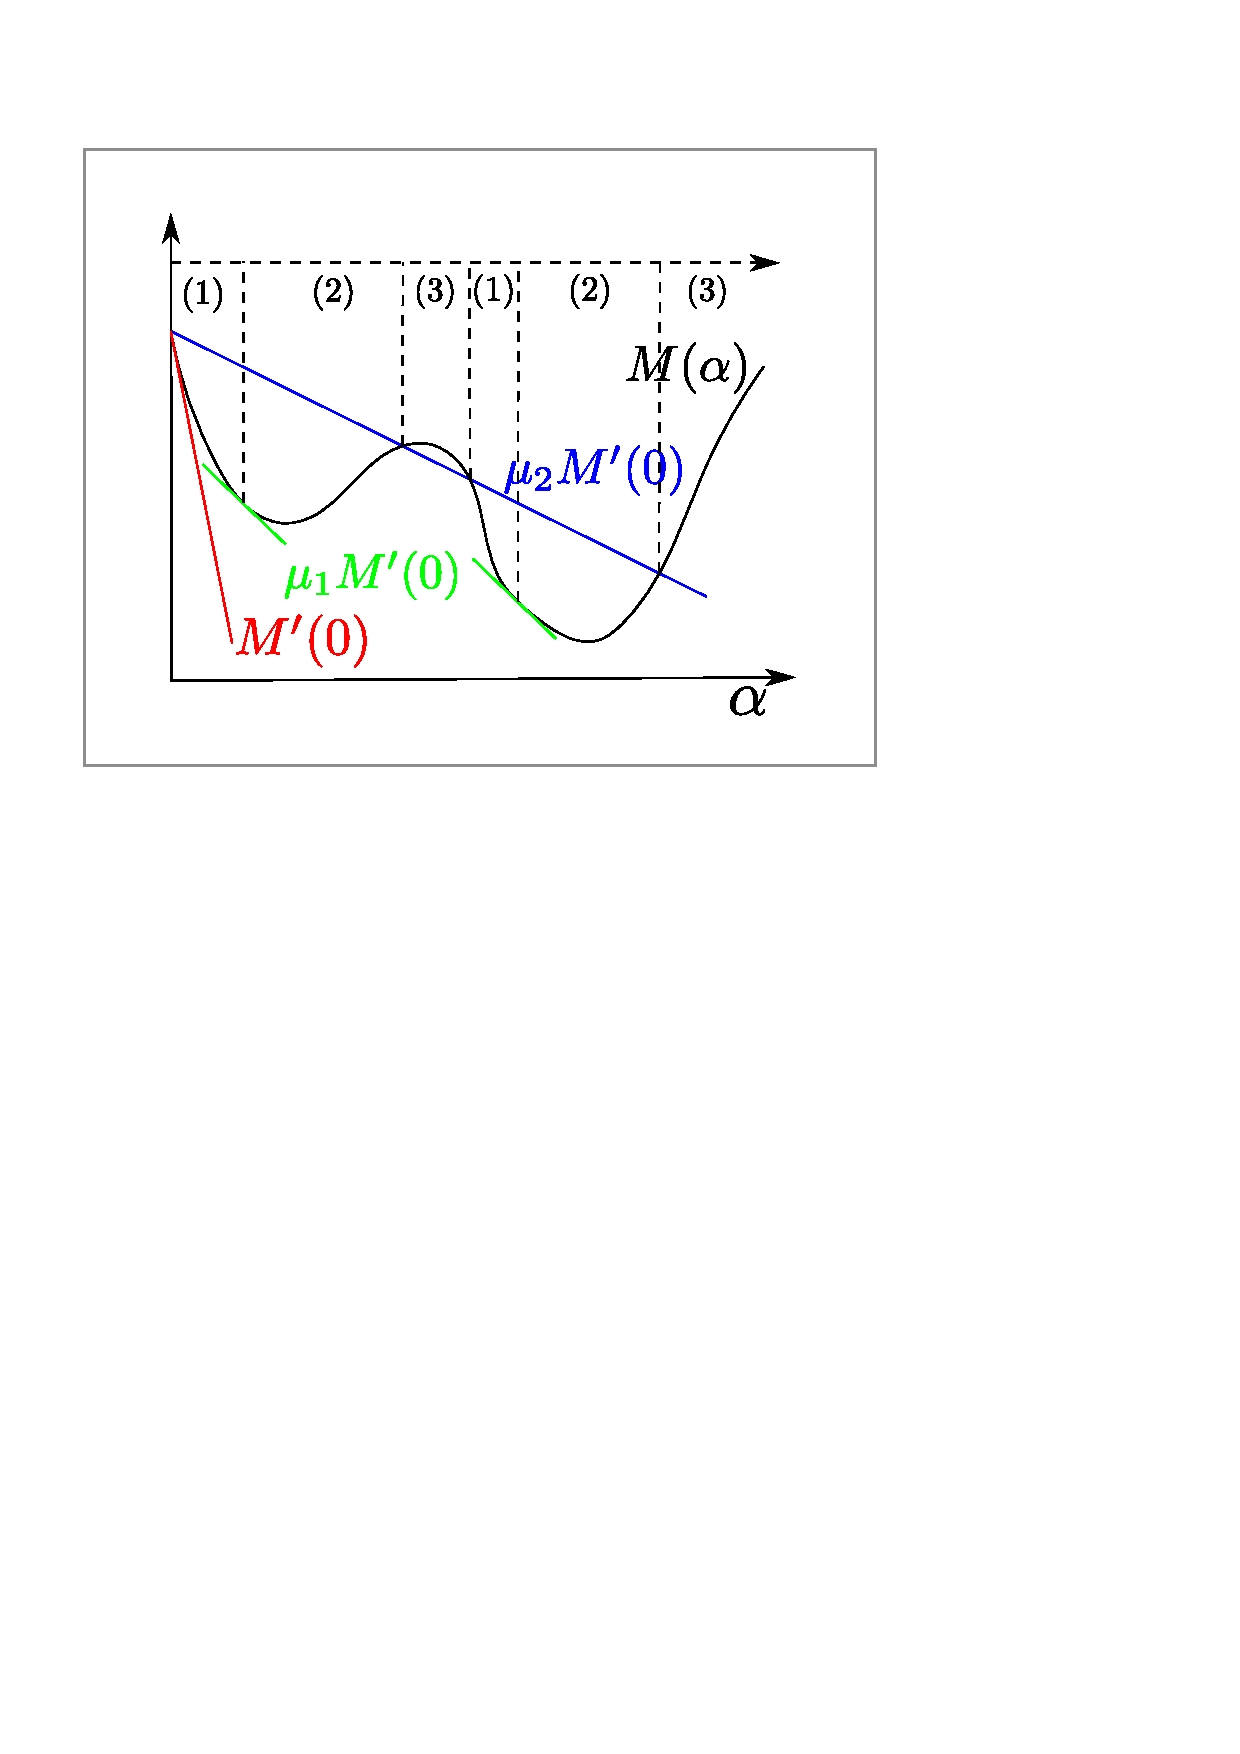
\includegraphics[width=0.7\textwidth]{line-search.pdf}
  \caption{Illustration of the choice made by the Wolfe line-search for values of $\alpha$}
\label{fig:Wolfe}
\end{figure}

The Wolfe line-search is popular, but it requires the computation of the derivative of the merit function, which can be prohibitively expensive in some cases, including in posture generation for robotics problems, where the derivatives are usually expensive.
Other line-search methods exist that do not require the derivative of $M$ for $\alpha\neq0$. For example the Goldstein and Price, or the Armijo methods.

\subsubsection{The filter method}
\label{ssub:the_filter_method}
The decision to accept on not a step generated by the QP can be made using a Filter approach instead of the Wolfe line search, as introduced by Fletcher in~\cite{fletcher:mathprog:2000}.
The goal of that method is to minimize the cost function $f(x)$ and the constraint violation $h(x)$ separately.
A step is accepted if it improves at least one of the function or the constraint violation.
\begin{equation}
  h(x) = \sum\limits_{k\in E} |c_k(x)| + \sum\limits_{k\in I} \max(0, -c_k(x))
\end{equation}

Denoting $h_i = h(x_i)$ and $f_i = f(x_i)$, we define the notion of domination as follows:
\begin{definition}
  \begin{equation}
    p_i\ \text{dominates }p_j \Leftrightarrow \left\{
        \begin{array}{l}
    f_i < f_j \\
    h_i < h_j
  \end{array}  \right.
  \end{equation}
\end{definition}

The filter maintains a list of pairs $p_i=\{f_i, h_i\}$ such that no pair dominates any other pair.
When a new point $x$ is submitted to the filter for acceptance, the values $f(x)$ and $h(x)$ are computed and the pair $p = \{f(x), h(x)\}$ is compared to every pairs $p_i$.
If there is at least one pair $p_i$ in the filter that dominates $p$, the point is refused.
Otherwise, no pair of the filter dominates $p$, then $p$ is accepted and added to the filter.
Once $p$ is added to the filter, any pair in the filter that is dominated by $p$ is removed from it to ensure to keep a list of pairs non dominated by each other in the filter.
In order to ensure global convergence, this method requires several refinements as explained in~\cite{fletcher:mathprog:2000}.
First, it needs to avoid accepting pairs that are excessively close to each other. For that, the domination criterion is modified with a sloping envelope, as proposed in Chin~\cite{chin:mathprog:2003}.
The sloping envelope definition takes user defined parameters $\beta$ and $\gamma$ in $[0,\ 1]$.

\begin{definition}
  \begin{equation}
    p_i\ \text{dominates }p_j \Leftrightarrow \left\{
        \begin{array}{l}
    f_i < f_j - \gamma h\ \\
    h_i < \beta h_j
  \end{array}  \right.
  \end{equation}
\end{definition}

\begin{figure}
  \centering
  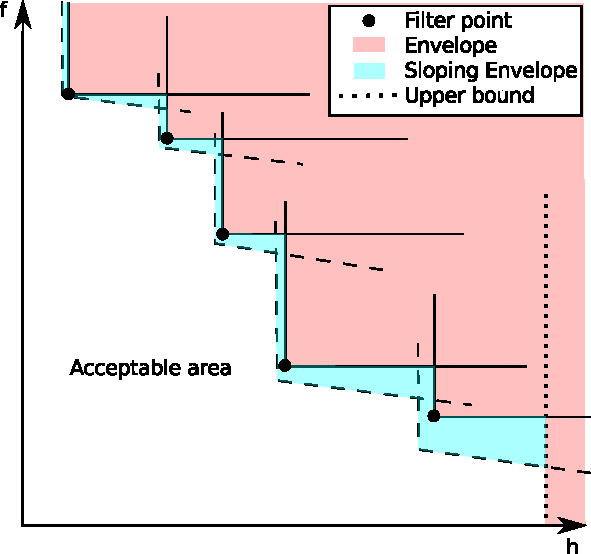
\includegraphics[width=0.7\textwidth]{filter.pdf}
  \caption{Representation of a filter with sloping envelope}
\label{fig:Filter}
\end{figure}

Another basic necessary improvement is to set an upper bound to the constraint violation, to avoid having the algorithm generate points that minimize the cost function while completely violating the constraints.

A representation of the filter method is given in figure~\ref{fig:Filter}

The filter method is convenient because it does not require the same complicated updates as can be found in penalty based methods where the penalty parameter needs to be updated regularly.
Also, with the filter method, no derivative computation is required.
That method is generally more permissive than merit based method in the sense that it refuses less points.

The filter method, as well as the merit function based methods can be used in line-search and trust-region algorithms.

\subsubsection{The Trust-Region Strategy}
\label{ssub:the_trust_region_strategy}
The Trust Region strategy is based on the idea that at any iterate $x_k$ the quadratic model made of the problem and fed to the QP solver can only be trusted to be relevant is a finite region around the iterate.
That region is called the trust region and its size is usually governed by a single positive parameter $\rho_k$ that can evolve along the optimization process.
This translates in a modified QP to solve at each iteration.
A boundary constraint describing the trust region is added to the problem.
At each step, the modified problem writes as:

\begin{equation}
  \begin{array}{ll}
    \minimize\limits_{z\in \mathbb{R}^n}{} & \frac{1}{2}z^T\nabla_{xx}^2Hz + \sum_{i\in\mathcal{U}}{\nabla c_i(x_k)}^T z \\
    \text{subject to } & {\nabla c_i(x_k)}^T z+c_i(x_k)=0,\ i\in \mathcal{F} \\
                       & {\nabla c_i(x_k)}^T z+c_i(x_k)\geq 0,\ i\in I\\
                       & |z|<\rho_k
  \end{array}
\label{approx_QP_TR}
\end{equation}

Once a solution $z$ of~\ref{approx_QP_TR} is found, the potential next iterate $x_{k+1} = x_k + z$ is checked against the acceptance criterion (should it be a merit function or a filter or other).
If it is accepted, that means that our current model is good, we move to the next step with $x_{k+1} \leftarrow x_k + z$, and the size of the trust region can be augmented based on some heuristics.
Otherwise, the iterate is refused, the model is less good than expected, the size of the trust region is reduced based on some heuristics (e.g. $\rho_{k+1}\leftarrow\rho_k /2$) and the problem~\ref{approx_QP_TR} is solved again with the new value of $\rho_{k+1}$.
This is repeated until a satisfying point is found, or until an infeasible problem is found.

\begin{figure}
  \centering
  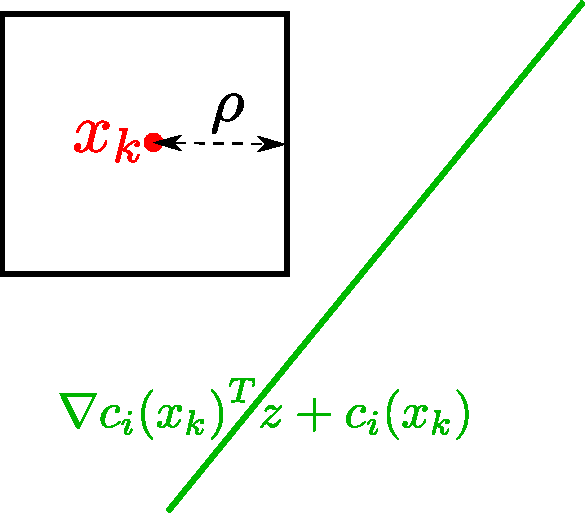
\includegraphics[width=0.4\textwidth]{trust_region_incompatible.pdf}
  \caption{Constraint incompatibility generated by trust region approach}
\label{fig:TR_incompatible}
\end{figure}

With this approach, a problem that often arises is the generation of infeasible problems.
The reduction of the size of the trust region can lead to an incompatible set of constraints.
For example, with a single constraint, as illustrated in figure~\ref{fig:TR_incompatible}.
The linearisation of the constraint is represented by the green line, and the trust region by the black rectangle.
If $\rho$ is too small, there is no intersection between the linearization of the constraint and the trust region.
The QP is then infeasible.
An obvious solution for that would be to increase the size of the trust region, but that goes against the core idea of the trust region strategy and it would harm the convergence properties of the algorithm.
A more appropriate solution is to enter a restoration phase when that event occur.
The purpose of a restoration phase is to reduce the infeasibility of a problem by relaxing infeasible constraints without regards for the cost function.
The restoration phase is exited once a feasible point is found, and the course of the SQP is continued from that point.

\subsection{Restoration phase}
\label{sub:restoration_phase}

As we stated previously, a restoration phase is entered when an infeasible problem is found by the trust region strategy.
The goal of the restoration is to find a solution to the following problem:

\begin{equation}
    \text{Find $x\in\mathbb{R}^n$ such that }
    \left\{
    \begin{array}{l}
      c_i(x)=0,\ i\in E \\
      c_i(x)\geq 0,\ i\in I\\
      |z|<\rho_k
    \end{array}
    \right.
\label{eq:resto_NL}
\end{equation}

The restoration phase proceeds in a similar way to the original SQP algorithm described earlier.
At each step, an approximated QP is solved, then its result is compared to an acceptance criterion, if it is accepted, the trust region can be increased and the algorithm continue.
Otherwise, the trust region is reduced and the problem is solved again.
The acceptance criterion must be tailored for the restoration problem, meaning that it is based on the values of the cost function of the restoration problem and of its constraints.
The big difference comes from the way the quadratic problem is constructed during this phase.

During a restoration phase step, the first action is to estimate the sets $\mathcal{F}$ and $\mathcal{I}$ of feasible  and infeasible constraints.
This is done by solving the linearization of problem~\Eqref{eq:resto_NL} as presented in~\Eqref{eq:FP}.
Each equality constraint is cut in 2 inequality constraints.

\begin{equation}
  \text{Find $z\in\mathbb{R}^n$ such that }
  \left\{
  \begin{array}{l}
    {\nabla c_i(x_k)}^T z+c_i(x_k)\geq 0,\ i\in E \\
    -{\nabla c_i(x_k)}^T z-c_i(x_k)\geq 0,\ i\in E \\
    {\nabla c_i(x_k)}^T z+c_i(x_k)\geq 0,\ i\in I\\
    |z|<\rho_k
  \end{array}
  \right.
\label{eq:FP}
\end{equation}

The resolution of that FP gives the lists $\mathcal{F}$ and $\mathcal{I}$.
If the list of infeasible constraints is empty, the problem is feasible, so the restoration phase is exited to return to the main SQP algorithm.
The restoration QP to solve is built based on those lists.
The infeasible constraints are removed from the constraint set and the expression of their violation is added to the cost function, while the feasible constraints remain in the constraint list.
This results in a problem like~\ref{rest_SQP} to solve.
(Note that the indexes of the constraints are modified to account for the duplication of the equality constraints)

\begin{equation}
  \begin{array}{ll}
    \minimize\limits_{z\in \mathbb{R}^n}{} & \frac{1}{2} z^T Hz - \sum\limits_{i\in\mathcal{I}}{\nabla c_i(x_k)}^T z \\
    \text{subject to } & {\nabla c_i(x_k)}^T z+c_i(x_k)\geq 0,\ i \in \mathcal{F} \\
                       & |z|<\rho_k
  \end{array}
\label{rest_SQP}
\end{equation}

This problem is solved by a QP solver, its result is checked against an acceptance criterion, based on that, the trust region is enlarged or reduced, and we go back to solving the FP\@.

In the restoration phase, special care must be taken in the computation of the matrix H, that represents the Hessian of the Lagrangian of a problem that changes at each iteration.
One possible approach is to compute it as the sum of the Hessians of all the individual constraints, and those can be computed exactly or with a quasi-newton approximation.


\subsection{Quasi-Newton Approximation}
\label{sub:quasi_newton_approximation}

In the SPQ algorithm, it is necessary to have access to the Hessian of the Lagrangian $\nabla_{xx}^2\mathcal{L}$ to be able to devise the QP subproblem to solve.
%For some strategies like the Line-Search, it is necessary that $\nabla_{xx}^2\mathcal{L}$ is definite positive.
Sometimes the exact Hessian of the problem is not positive definite.
Also it is often difficult or computationally expensive to compute an exact Hessian of the Lagrangian.
Since we are following an iterative process, it is not necessary to have an exact knowledge of the Hessian and using an approximation of it is usually enough.
Also, an approximate Hessian is in most cases less expensive to compute than the exact one.

The idea behind computing an approximate Hessian is that, starting from an initial approximate Hessian $B_0$, we compute at each iteration an update to the approximate Hessian based on the values and first order derivatives of the Lagrangian.
This update aims at capturing some curvature information about the Hessian by evaluating the evolution of the gradient along the latest step.
At step $k$, the Hessian update is a function of $s_k$ and $y_k$:
\begin{equation}
  s_k = x_{k+1}-x_k,\ \ \ \
  y_k = \nabla_x\mathcal{L}(x_{k+1}, \lambda_{k+1}) - \nabla_x\mathcal{L}(x_{k}, \lambda_{k+1})
\end{equation}

The two most famous Hessian update strategies are called the BFGS (Broyden–Fletcher– Goldfarb–Shanno) and the SR1(Symmetric Rank 1) updates.
BFGS is a rank 2 update while SR1 is rank 1.

The most basic formulas for the BFGS update is the following:

\begin{equation}
\label{BFGS}
  B_{k+1} = B_k - \frac{B_k s_k s_k^T B_k}{s_k^T B_k s_k} + \frac{y_k y_k^T}{s_k^T y_k}
\end{equation}

Note that using a BFGS update requires that $s_k$ and $y_k$ satisfy the curvature condition: $s_k^T y_k>0$.
If that condition does not hold, then the value of $y_k$ is modified, which gives rise to the Damped BFGS update, which guarantees to keep $B_k$ definite positive:

\begin{equation}
\label{damped_BFGS}
\begin{split}
  \theta_k =
  \left\{
      \begin{array}{ll}
      1 & \text{if } s_k^T y_k \geq 0.2 s_k^T B_k s_k \\
      \frac{0.8 s_k^T B_k s_k}{s_k^T B_k s_k-s_k^T y_k} & \text{if } s_k^T y_k \geq 0.2s_k^T B_k s_k \\
      \end{array}
      \right.\\
      r_k = \theta_k y_k + (1-\theta_k) B_k s_k\\
      B_{k+1} = B_k-\frac{B_k s_k s_k^T B_k}{s_k^T B_k s_k} + \frac{r_k r_k^T}{s_k^T r_k}
\end{split}
\end{equation}

The SR1 update is computed with the following formula:

\begin{equation}
\label{SR1}
B_{k+1} = B_k + \frac{(y_k-B_k s_k){(y_k-B_k s_k)}^T}{{(y_k-B_k s_k)}^T s_k}
\end{equation}

Both those formulas proved to be efficient in some cases. It is not yet clear in which cases one is better than the other.

\section{Conclusion}
This section gives a general introduction to nonlinear constrained optimization without regards for robotics or optimization on manifolds

